%
%DIF LATEXDIFF DIFFERENCE FILE
%DIF DEL slides_origin.tex   Sat Apr 24 09:04:00 2021
%DIF ADD slides.tex          Fri Apr 23 23:36:37 2021
% ---------------------------------------------------------------
% Copyright (C) 2012-2018 Gang Li
% ---------------------------------------------------------------
%
% This work is the default powerdot-tuliplab style test file and may be
% distributed and/or modified under the conditions of the LaTeX Project Public
% License, either version 1.3 of this license or (at your option) any later
% version. The latest version of this license is in
% http://www.latex-project.org/lppl.txt and version 1.3 or later is part of all
% distributions of LaTeX version 2003/12/01 or later.
%
% This work has the LPPL maintenance status "maintained".
%
% This Current Maintainer of this work is Gang Li.
%
%latex slides.tex 
%dvips slides.dvi
%ps2pdf slides.ps
\documentclass[
 size=14pt,
 paper=smartboard,  %a4paper, smartboard, screen
 mode=present, 		%present, handout, print
 display=slides, 	% slidesnotes, notes, slides
 style=tuliplab,  	% TULIP Lab style
 pauseslide,
 fleqn,leqno]{powerdot}

\usepackage{cancel}
\usepackage{caption}
\usepackage{stackengine}
\usepackage{smartdiagram}
\usepackage{attrib}
\usepackage{amssymb}
\usepackage{amsmath} 
\usepackage{amsthm} 
\usepackage{mathtools}
\usepackage{rotating}
\usepackage{graphicx}
\usepackage{boxedminipage}
\usepackage{rotate}
\usepackage{calc}
\usepackage[absolute]{textpos}
\usepackage{psfrag,overpic}
\usepackage{fouriernc}
\usepackage{pstricks,pst-3d,pst-grad,pstricks-add,pst-text,pst-node,pst-tree}
\usepackage{moreverb,epsfig,subfigure}
\usepackage{color}
\usepackage{booktabs}
\usepackage{etex}
\usepackage{breqn}
\usepackage{multirow}
\usepackage{natbib}
\usepackage{bibentry}
\usepackage{gitinfo2}
\usepackage{siunitx}
\usepackage{nicefrac}
\usepackage{media9}
\usepackage{animate}
\usepackage{auto-pst-pdf}
\usepackage{breakurl}
\usepackage{fontawesome}
\usepackage{xcolor}
\usepackage{multicol}



\usepackage{verbatim}
\usepackage[utf8]{inputenc}
\usepackage{dtk-logos}
\usepackage{tikz}
\usepackage{adigraph}
\usepackage{hyperref}
\usepackage{pgfplots}
\usepackage{verbatim}
\usepackage{fontawesome}


\usepackage{todonotes}
\usepackage{animate}
\usepackage{fontawesome}

\usepackage{listings}
\lstset{frameround=fttt,
frame=trBL,
stringstyle=\ttfamily,
backgroundcolor=\color{yellow!20},
basicstyle=\footnotesize\ttfamily}
\lstnewenvironment{code}{
\lstset{frame=single,escapeinside=`',
backgroundcolor=\color{yellow!20},
basicstyle=\footnotesize\ttfamily}
}{}


\usepackage{hyperref}
\hypersetup{ % TODO: PDF meta Data
  pdftitle={Presentation Title},
  pdfauthor={Gang Li},
  pdfpagemode={FullScreen},
  pdfborder={0 0 0}
}


% \usepackage{auto-pst-pdf}
% package to show source code

\definecolor{LightGray}{rgb}{0.9,0.9,0.9}
\newlength{\pixel}\setlength\pixel{0.000714285714\slidewidth}
\setlength{\TPHorizModule}{\slidewidth}
\setlength{\TPVertModule}{\slideheight}
\newcommand\highlight[1]{\fbox{#1}}
\newcommand\icite[1]{{\footnotesize [#1]}}

\newcommand\twotonebox[2]{\fcolorbox{pdcolor2}{pdcolor2}
{#1\vphantom{#2}}\fcolorbox{pdcolor2}{white}{#2\vphantom{#1}}}
\newcommand\twotoneboxo[2]{\fcolorbox{pdcolor2}{pdcolor2}
{#1}\fcolorbox{pdcolor2}{white}{#2}}
\newcommand\vpspace[1]{\vphantom{\vspace{#1}}}
\newcommand\hpspace[1]{\hphantom{\hspace{#1}}}
\newcommand\COMMENT[1]{}

\newcommand\placepos[3]{\hbox to\z@{\kern#1
        \raisebox{-#2}[\z@][\z@]{#3}\hss}\ignorespaces}

\renewcommand{\baselinestretch}{1.2}


\newcommand{\draftnote}[3]{
	\todo[author=#2,color=#1!30,size=\footnotesize]{\textsf{#3}}	}
% TODO: add yourself here:
%
\newcommand{\gangli}[1]{\draftnote{blue}{GLi:}{#1}}
\newcommand{\shaoni}[1]{\draftnote{green}{sn:}{#1}}
\newcommand{\gliMarker}
	{\todo[author=GLi,size=\tiny,inline,color=blue!40]
	{Gang Li has worked up to here.}}
\newcommand{\snMarker}
	{\todo[author=Sn,size=\tiny,inline,color=green!40]
	{Shaoni has worked up to here.}}

%%%%%%%%%%%%%%%%%%%%%%%%%%%%%%%%%%%%%%%%%%%%%%%%%%%%%%%%%%%%%%%%%%%%%%%%
% title
% TODO: Customize to your Own Title, Name, Address
%
\title{Predict future sales}
\author{
Pengcheng Jiang
\\
\\JiLin University
}
\date{\gitCommitterDate}


% Customize the setting of slides
\pdsetup{
% TODO: Customize the left footer, and right footer
rf=\href{http://www.tulip.org.au}{
Last Changed by: \textsc{\gitCommitterName}\ \gitVtagn-\gitAbbrevHash\ (\gitAuthorDate)
},
cf={Predict future sales},
}
%DIF PREAMBLE EXTENSION ADDED BY LATEXDIFF
%DIF UNDERLINE PREAMBLE %DIF PREAMBLE
\RequirePackage[normalem]{ulem} %DIF PREAMBLE
\RequirePackage{color}\definecolor{RED}{rgb}{1,0,0}\definecolor{BLUE}{rgb}{0,0,1} %DIF PREAMBLE
\providecommand{\DIFaddtex}[1]{{\protect\color{blue}\uwave{#1}}} %DIF PREAMBLE
\providecommand{\DIFdeltex}[1]{{\protect\color{red}\sout{#1}}}                      %DIF PREAMBLE
%DIF SAFE PREAMBLE %DIF PREAMBLE
\providecommand{\DIFaddbegin}{} %DIF PREAMBLE
\providecommand{\DIFaddend}{} %DIF PREAMBLE
\providecommand{\DIFdelbegin}{} %DIF PREAMBLE
\providecommand{\DIFdelend}{} %DIF PREAMBLE
\providecommand{\DIFmodbegin}{} %DIF PREAMBLE
\providecommand{\DIFmodend}{} %DIF PREAMBLE
%DIF FLOATSAFE PREAMBLE %DIF PREAMBLE
\providecommand{\DIFaddFL}[1]{\DIFadd{#1}} %DIF PREAMBLE
\providecommand{\DIFdelFL}[1]{\DIFdel{#1}} %DIF PREAMBLE
\providecommand{\DIFaddbeginFL}{} %DIF PREAMBLE
\providecommand{\DIFaddendFL}{} %DIF PREAMBLE
\providecommand{\DIFdelbeginFL}{} %DIF PREAMBLE
\providecommand{\DIFdelendFL}{} %DIF PREAMBLE
%DIF HYPERREF PREAMBLE %DIF PREAMBLE
\providecommand{\DIFadd}[1]{\texorpdfstring{\DIFaddtex{#1}}{#1}} %DIF PREAMBLE
\providecommand{\DIFdel}[1]{\texorpdfstring{\DIFdeltex{#1}}{}} %DIF PREAMBLE
\newcommand{\DIFscaledelfig}{0.5}
%DIF HIGHLIGHTGRAPHICS PREAMBLE %DIF PREAMBLE
\RequirePackage{settobox} %DIF PREAMBLE
\RequirePackage{letltxmacro} %DIF PREAMBLE
\newsavebox{\DIFdelgraphicsbox} %DIF PREAMBLE
\newlength{\DIFdelgraphicswidth} %DIF PREAMBLE
\newlength{\DIFdelgraphicsheight} %DIF PREAMBLE
% store original definition of \includegraphics %DIF PREAMBLE
\LetLtxMacro{\DIFOincludegraphics}{\includegraphics} %DIF PREAMBLE
\newcommand{\DIFaddincludegraphics}[2][]{{\color{blue}\fbox{\DIFOincludegraphics[#1]{#2}}}} %DIF PREAMBLE
\newcommand{\DIFdelincludegraphics}[2][]{% %DIF PREAMBLE
\sbox{\DIFdelgraphicsbox}{\DIFOincludegraphics[#1]{#2}}% %DIF PREAMBLE
\settoboxwidth{\DIFdelgraphicswidth}{\DIFdelgraphicsbox} %DIF PREAMBLE
\settoboxtotalheight{\DIFdelgraphicsheight}{\DIFdelgraphicsbox} %DIF PREAMBLE
\scalebox{\DIFscaledelfig}{% %DIF PREAMBLE
\parbox[b]{\DIFdelgraphicswidth}{\usebox{\DIFdelgraphicsbox}\\[-\baselineskip] \rule{\DIFdelgraphicswidth}{0em}}\llap{\resizebox{\DIFdelgraphicswidth}{\DIFdelgraphicsheight}{% %DIF PREAMBLE
\setlength{\unitlength}{\DIFdelgraphicswidth}% %DIF PREAMBLE
\begin{picture}(1,1)% %DIF PREAMBLE
\thicklines\linethickness{2pt} %DIF PREAMBLE
{\color[rgb]{1,0,0}\put(0,0){\framebox(1,1){}}}% %DIF PREAMBLE
{\color[rgb]{1,0,0}\put(0,0){\line( 1,1){1}}}% %DIF PREAMBLE
{\color[rgb]{1,0,0}\put(0,1){\line(1,-1){1}}}% %DIF PREAMBLE
\end{picture}% %DIF PREAMBLE
}\hspace*{3pt}}} %DIF PREAMBLE
} %DIF PREAMBLE
\LetLtxMacro{\DIFOaddbegin}{\DIFaddbegin} %DIF PREAMBLE
\LetLtxMacro{\DIFOaddend}{\DIFaddend} %DIF PREAMBLE
\LetLtxMacro{\DIFOdelbegin}{\DIFdelbegin} %DIF PREAMBLE
\LetLtxMacro{\DIFOdelend}{\DIFdelend} %DIF PREAMBLE
\DeclareRobustCommand{\DIFaddbegin}{\DIFOaddbegin \let\includegraphics\DIFaddincludegraphics} %DIF PREAMBLE
\DeclareRobustCommand{\DIFaddend}{\DIFOaddend \let\includegraphics\DIFOincludegraphics} %DIF PREAMBLE
\DeclareRobustCommand{\DIFdelbegin}{\DIFOdelbegin \let\includegraphics\DIFdelincludegraphics} %DIF PREAMBLE
\DeclareRobustCommand{\DIFdelend}{\DIFOaddend \let\includegraphics\DIFOincludegraphics} %DIF PREAMBLE
\LetLtxMacro{\DIFOaddbeginFL}{\DIFaddbeginFL} %DIF PREAMBLE
\LetLtxMacro{\DIFOaddendFL}{\DIFaddendFL} %DIF PREAMBLE
\LetLtxMacro{\DIFOdelbeginFL}{\DIFdelbeginFL} %DIF PREAMBLE
\LetLtxMacro{\DIFOdelendFL}{\DIFdelendFL} %DIF PREAMBLE
\DeclareRobustCommand{\DIFaddbeginFL}{\DIFOaddbeginFL \let\includegraphics\DIFaddincludegraphics} %DIF PREAMBLE
\DeclareRobustCommand{\DIFaddendFL}{\DIFOaddendFL \let\includegraphics\DIFOincludegraphics} %DIF PREAMBLE
\DeclareRobustCommand{\DIFdelbeginFL}{\DIFOdelbeginFL \let\includegraphics\DIFdelincludegraphics} %DIF PREAMBLE
\DeclareRobustCommand{\DIFdelendFL}{\DIFOaddendFL \let\includegraphics\DIFOincludegraphics} %DIF PREAMBLE
%DIF LISTINGS PREAMBLE %DIF PREAMBLE
\RequirePackage{listings} %DIF PREAMBLE
\RequirePackage{color} %DIF PREAMBLE
\lstdefinelanguage{DIFcode}{ %DIF PREAMBLE
%DIF DIFCODE_UNDERLINE %DIF PREAMBLE
  moredelim=[il][\color{red}\sout]{\%DIF\ <\ }, %DIF PREAMBLE
  moredelim=[il][\color{blue}\uwave]{\%DIF\ >\ } %DIF PREAMBLE
} %DIF PREAMBLE
\lstdefinestyle{DIFverbatimstyle}{ %DIF PREAMBLE
	language=DIFcode, %DIF PREAMBLE
	basicstyle=\ttfamily, %DIF PREAMBLE
	columns=fullflexible, %DIF PREAMBLE
	keepspaces=true %DIF PREAMBLE
} %DIF PREAMBLE
\lstnewenvironment{DIFverbatim}{\lstset{style=DIFverbatimstyle}}{} %DIF PREAMBLE
\lstnewenvironment{DIFverbatim*}{\lstset{style=DIFverbatimstyle,showspaces=true}}{} %DIF PREAMBLE
%DIF END PREAMBLE EXTENSION ADDED BY LATEXDIFF

\begin{document}

\maketitle

\begin{slide}[toc=,bm=]{Overview}
\tableofcontents[content=currentsection,type=1]
\end{slide}

\section{Problem Definition}

%%==========================================================================================
%%
\begin{slide}[toc=,bm=]{Predict future sales}
  \begin{center}
    \DIFdelbegin %DIFDELCMD < \begin{itemize}
\begin{itemize}%DIFAUXCMD
%DIFDELCMD <   \item %%%
\item%DIFAUXCMD
\DIFdel{given: a challenging time-series dataset consisting of daily sales data, kindly provided by one of the largest Russian software firms - 1C Company.
  }%DIFDELCMD < \item %%%
\item%DIFAUXCMD
\DIFdel{target: predict total sales for every product and store in the next month
  }%DIFDELCMD < \item %%%
\item%DIFAUXCMD
\DIFdel{evaluation: Submissions are evaluated by root mean squared error (RMSE)
  }
\end{itemize}%DIFAUXCMD
%DIFDELCMD < \end{itemize}
%DIFDELCMD <   %%%
\DIFdelend \DIFaddbegin \twotonebox{\parbox{.1\textwidth}{given}}{\parbox{.76\textwidth}
    {
      a challenging time-series dataset consisting of daily sales data, kindly provided by one of the largest Russian software firms - 1C Company.
    }}
    \twotonebox{\parbox{.1\textwidth}{target}}{\parbox{.76\textwidth}
    {
      predict total sales for every product and store in the next month
    }}
    \twotonebox{\parbox{.1\textwidth}{evaluate}}{\parbox{.76\textwidth}
    {
      Submissions are evaluated by root mean squared error (RMSE)
    }}
  \DIFaddend \end{center}
\DIFaddbegin 

\DIFaddend \end{slide}
%%
%%==========================================================================================

\section{Data Cleaning}
\DIFaddbegin 


\DIFaddend %%==========================================================================================
%%
\begin{slide}[toc=,bm=]{Date}
\DIFdelbegin %DIFDELCMD < \begin{itemize}
\begin{itemize}%DIFAUXCMD
%DIFDELCMD <   \item %%%
\item%DIFAUXCMD
\DIFdel{item_categories.csv:item_category_name	item_category_id}%DIFDELCMD < \par
%DIFDELCMD <   \smallskip
%DIFDELCMD <   \item %%%
\item%DIFAUXCMD
\DIFdel{items.csv:item_id	item_category_id}%DIFDELCMD < \par
%DIFDELCMD <   \item %%%
\item%DIFAUXCMD
\DIFdel{sales_train.csv:date  date_block_num  shop_id  item_id  item_price item_cnt_day}%DIFDELCMD < \par
%DIFDELCMD <   \item %%%
\item%DIFAUXCMD
\DIFdel{shops.csv:shop_name	shop_id}%DIFDELCMD < \par
%DIFDELCMD <   \item %%%
\item%DIFAUXCMD
\DIFdel{test.csv:shop_id  item_id}%DIFDELCMD < \par

\end{itemize}%DIFAUXCMD
%DIFDELCMD < \end{itemize}
%DIFDELCMD < %%%
\DIFdelend \DIFaddbegin \begin{table}[h]
  \begin{center}
    \resizebox{\textwidth}{15mm}{
      \begin{tabular}{c| c c c c c c}
      \toprule
      File & \texttt{filed1}  & \texttt{filed2} & \texttt{filed3} & \texttt{filed4} & \texttt{filed5} & \texttt{filed6}\\
      \midrule
      item_categories
      &  item_category_name &  item_category_id \\
      items
      &  item_id &  item_category_id \\
      sales_train
      &  date & date_block_num &  shop_id  & item_id &  item_price &  item_cnt_day \\
      shops
      &  shop_name &  shop_id \\
      test
      &  shop_id &  item_id\\
      \bottomrule
      \end{tabular}
    }
  \end{center}
  \caption{\DIFaddFL{Data Infomation}}
\end{table}
\DIFaddend \end{slide}
%%
%%==========================================================================================


%%==========================================================================================
%%
\begin{slide}[toc=,bm=]{Data Information}
  \DIFdelbegin \DIFdel{sales_train:}%DIFDELCMD < \par
%DIFDELCMD <     \begin{itemize}
\begin{itemize}%DIFAUXCMD
%DIFDELCMD <       \item %%%
\item%DIFAUXCMD
\DIFdel{2935849 rows,6 columns
      }%DIFDELCMD < \item %%%
\item%DIFAUXCMD
\DIFdel{21807 items,60 shops
      }%DIFDELCMD < \item %%%
\item%DIFAUXCMD
\DIFdel{data_type
            }%DIFDELCMD < \begin{itemize}
%DIFDELCMD <               \item %%%
\item%DIFAUXCMD
\DIFdel{data: object
              }%DIFDELCMD < \item %%%
\item%DIFAUXCMD
\DIFdel{date_block_num: int
              }%DIFDELCMD < \item %%%
\item%DIFAUXCMD
\DIFdel{shop_id:int
              }%DIFDELCMD < \item %%%
\item%DIFAUXCMD
\DIFdel{item_id:int
              }%DIFDELCMD < \item %%%
\item%DIFAUXCMD
\DIFdel{item_price:float
              }%DIFDELCMD < \item %%%
\item%DIFAUXCMD
\DIFdel{item_cnt_day:float
            }
\end{itemize}%DIFAUXCMD
%DIFDELCMD < \end{itemize}
%DIFDELCMD <     \end{itemize}
%DIFDELCMD < %%%
\DIFdelend \DIFaddbegin \twotonebox{\parbox{.2\textwidth}{sales_train}}{\parbox{.76\textwidth}
  {
    \begin{itemize}
      \item 2935849 rows,6 columns
      \item 21807 items,60 shops
      \item data_type
            \begin{itemize}
              \item data: object
              \item date_block_num: int
              \item shop_id:int
              \item item_id:int
              \item item_price:float
              \item item_cnt_day:float
            \end{itemize}
    \end{itemize}
  }}
\DIFaddend \end{slide}
%%
%%==========================================================================================


%%==========================================================================================
%%
\begin{slide}[toc=,bm=]{Data Information}
  \DIFdelbegin \DIFdel{test:}%DIFDELCMD < \par
%DIFDELCMD <     \begin{itemize}
\begin{itemize}%DIFAUXCMD
%DIFDELCMD <       \item %%%
\item%DIFAUXCMD
\DIFdel{214200 rows,3 columns
      }%DIFDELCMD < \item %%%
\item%DIFAUXCMD
\DIFdel{5100 items,40 shops
      }%DIFDELCMD < \item %%%
\item%DIFAUXCMD
\DIFdel{data_type
            }%DIFDELCMD < \begin{itemize}
%DIFDELCMD <               \item %%%
\item%DIFAUXCMD
\DIFdel{ID:int
              }%DIFDELCMD < \item %%%
\item%DIFAUXCMD
\DIFdel{shop_id:int
              }%DIFDELCMD < \item %%%
\item%DIFAUXCMD
\DIFdel{item_id:int
            }
\end{itemize}%DIFAUXCMD
%DIFDELCMD < \end{itemize}
%DIFDELCMD <     \end{itemize}
%DIFDELCMD <     %%%
\DIFdel{From here you can see a lot of stores, goods in training set are not in the test set
}\DIFdelend \DIFaddbegin \twotonebox{\parbox{.2\textwidth}{test}}{\parbox{.76\textwidth}
  {
    \begin{itemize}
      \item 214200 rows,3 columns
      \item 5100 items,40 shops
      \item data_type
            \begin{itemize}
              \item ID:int
              \item shop_id:int
              \item item_id:int
            \end{itemize}
    \end{itemize}
    From here you can see a lot of stores, goods in training set are not in the test set
  }}
\DIFaddend \end{slide}
%%
%%==========================================================================================



%%==========================================================================================
%%
\begin{slide}[toc=,bm=]{Missing Value and Non Value}
  \DIFdelbegin \DIFdel{target:Find out whether there are empty values or missing values in the data}%DIFDELCMD < \par
%DIFDELCMD <   %%%
\DIFdel{result:}%DIFDELCMD < \par
%DIFDELCMD <   %%%
\DIFdel{missing value:0}%DIFDELCMD < \par
%DIFDELCMD <   %%%
\DIFdel{nan value:0}%DIFDELCMD < \par
%DIFDELCMD < %%%
\DIFdelend \DIFaddbegin \twotonebox{\parbox{.1\textwidth}{target}}{\parbox{.76\textwidth}
  {
    Find out whether there are empty values or missing values in the data
  }}
  \twotonebox{\parbox{.1\textwidth}{result}}{\parbox{.76\textwidth}
  {
    \begin{itemize}
      \item   missing value:0
      \item   nan value:0
    \end{itemize}
  }}
\DIFaddend \end{slide}
%%
%%==========================================================================================

%%==========================================================================================
%%
\DIFdelbegin %DIFDELCMD < \begin{slide}[toc=,bm=]{Data leakages}
%DIFDELCMD <   %%%
\DIFdel{target:delete stores, goods in training set but not in the test set}%DIFDELCMD < \par
%DIFDELCMD <   %%%
\DIFdel{result:}%DIFDELCMD < \par
%DIFDELCMD <   \setlength\parindent{2em}%%%
\DIFdel{sales_train}%DIFDELCMD < \par
%DIFDELCMD <   \setlength\parindent{4em}%%%
\DIFdel{rows:1224439}%DIFDELCMD < \par
%DIFDELCMD <     \setlength\parindent{4em}%%%
\DIFdel{items:4716}%DIFDELCMD < \par
%DIFDELCMD <     \setlength\parindent{4em}%%%
\DIFdel{shops:42}%DIFDELCMD < \par
%DIFDELCMD < %%%
\DIFdelend \DIFaddbegin \begin{slide}[toc=,bm=]{Cartesian product}
  \twotonebox{\parbox{.1\textwidth}{reason}}{\parbox{.76\textwidth}
  {
    The training set contains only the items that the store actually sold that month
  }}
  \twotonebox{\parbox{.1\textwidth}{target}}{\parbox{.76\textwidth}
  {
    for items not sold during the month, you should add them and set them to 0(Find out all the stores and merchandise, and make cartesian product with sales_trainz)
  }}

\DIFaddend \end{slide}
%%
%%==========================================================================================


%%==========================================================================================
%%
\DIFdelbegin %DIFDELCMD < \begin{slide}[toc=,bm=]{Data duplication}
%DIFDELCMD <   %%%
\DIFdel{target:See if duplicate items exist in the dataset}%DIFDELCMD < \par
%DIFDELCMD <   %%%
\DIFdel{result:}%DIFDELCMD < \par
%DIFDELCMD <     \setlength\parindent{2em}%%%
\DIFdel{sales_train:6}%DIFDELCMD < \par
%DIFDELCMD <     \setlength\parindent{2em}%%%
\DIFdel{test:0}%DIFDELCMD < \par
%DIFDELCMD <   %%%
\DIFdel{operation:delete duplications
}\DIFdelend \DIFaddbegin \begin{slide}[toc=,bm=]{Data leakages}
  \twotonebox{\parbox{.1\textwidth}{target}}{\parbox{.76\textwidth}
  {
    delete stores, goods in training set but not in the test set
  }}
  \twotonebox{\parbox{.1\textwidth}{result}}{\parbox{.76\textwidth}
  {
    \begin{itemize}
      \item sales_train:
      \item rows:1224439
      \item items:4716
      \item shops:42
    \end{itemize}
    %\setlength\parindent{2em}sales_train\par
  }}
\DIFaddend \end{slide}
%%
%%==========================================================================================


%%==========================================================================================
%%
\DIFdelbegin %DIFDELCMD < \begin{slide}[toc=,bm=]{Outliers}
%DIFDELCMD <   %%%
\DIFdel{target:Calculate the outliers of item_cnt_day and item price}%DIFDELCMD < \par
%DIFDELCMD <   %%%
\DIFdel{result:
}\DIFdelend \DIFaddbegin \begin{slide}[toc=,bm=]{Data duplication}
  \twotonebox{\parbox{.1\textwidth}{target}}{\parbox{.76\textwidth}
  {
    See if duplicate items exist in the dataset
  }}
  \twotonebox{\parbox{.1\textwidth}{result}}{\parbox{.76\textwidth}
  {
    \begin{itemize}
      \item sales_train:6
      \item test:0
    \end{itemize}
  }}
\DIFaddend \end{slide}
%%
%%==========================================================================================

%%==========================================================================================
%%
\begin{slide}[toc=,bm=]{Outliers}
  \DIFdelbegin %DIFDELCMD < \begin{figure}
%DIFDELCMD <     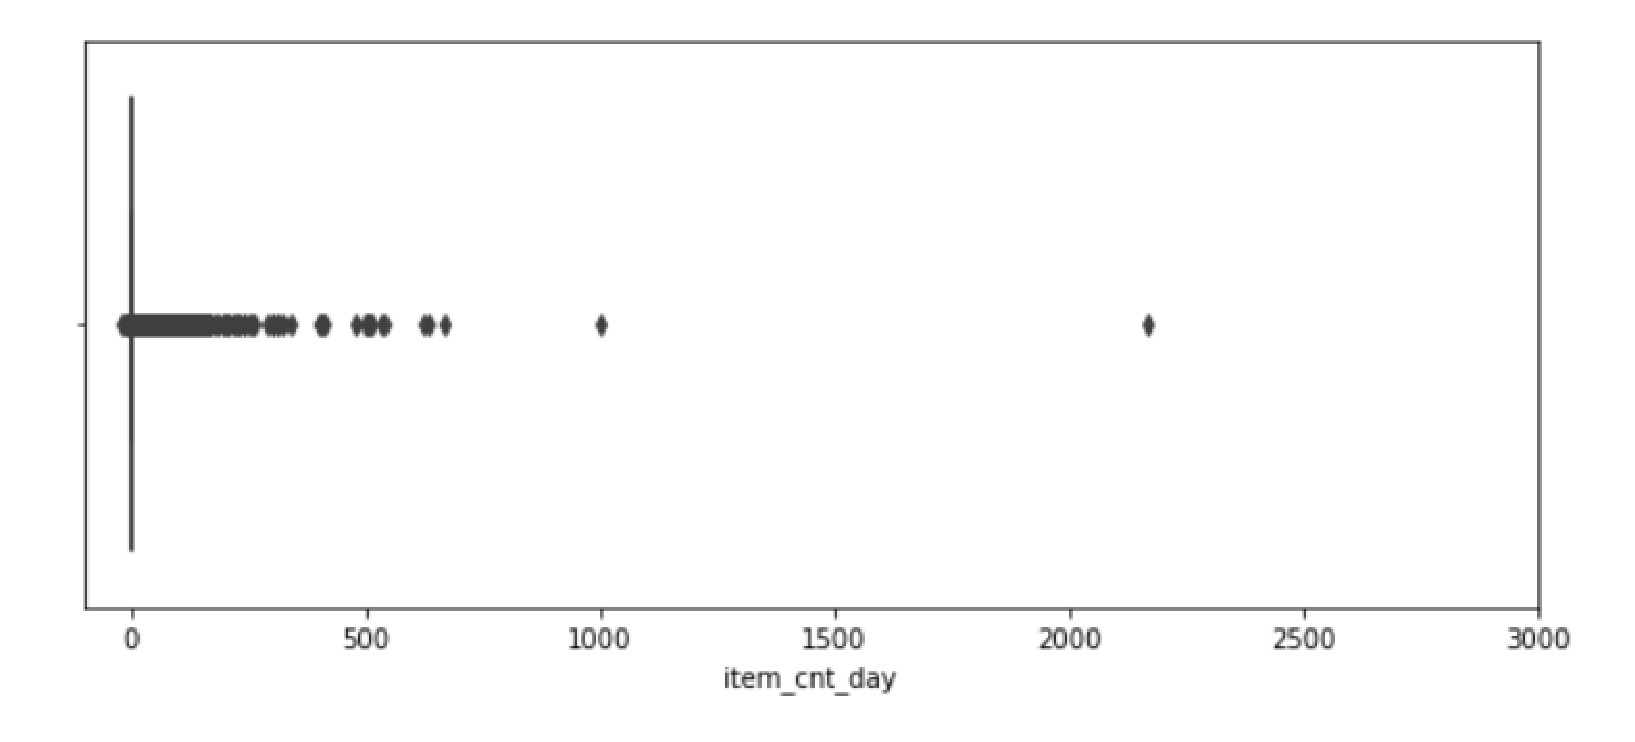
\includegraphics[scale=0.5]{picture/data_7.eps}
%DIFDELCMD <   \end{figure}
%DIFDELCMD < %%%
\DIFdelend \DIFaddbegin \twotonebox{\parbox{.1\textwidth}{target}}{\parbox{.76\textwidth}
  {
    Calculate the outliers of item_cnt_day and item price
  }}
  \twotonebox{\parbox{.1\textwidth}{result}}{\parbox{.76\textwidth}
  {
    \begin{figure}
      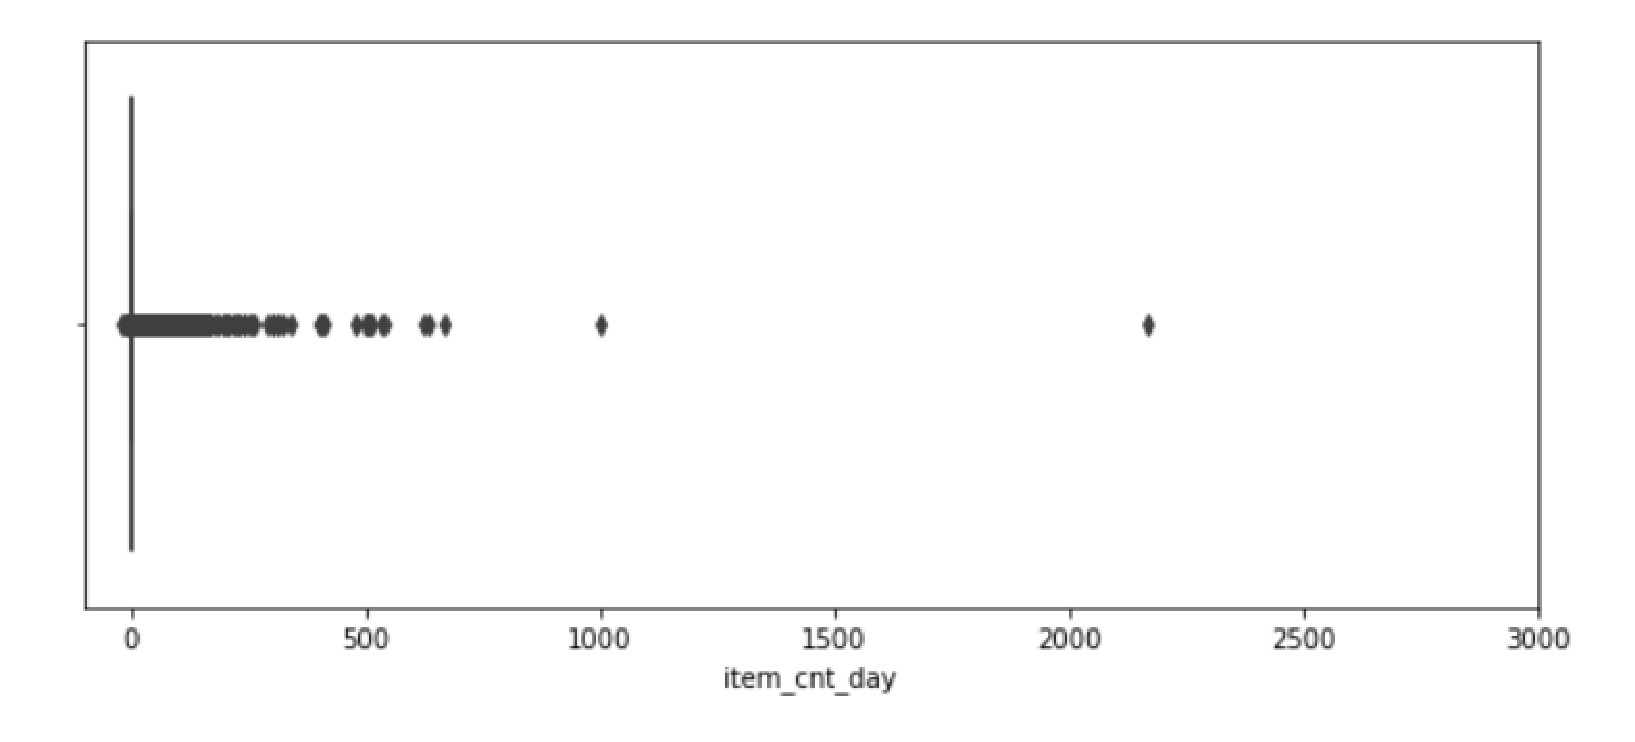
\includegraphics[scale=0.5]{picture/data_7.eps}
    \end{figure}
  }}
\DIFaddend \end{slide}
%%
%%==========================================================================================

%%==========================================================================================
%%
\begin{slide}[toc=,bm=]{Outliers}
  \DIFdelbegin %DIFDELCMD < \begin{figure}
%DIFDELCMD <     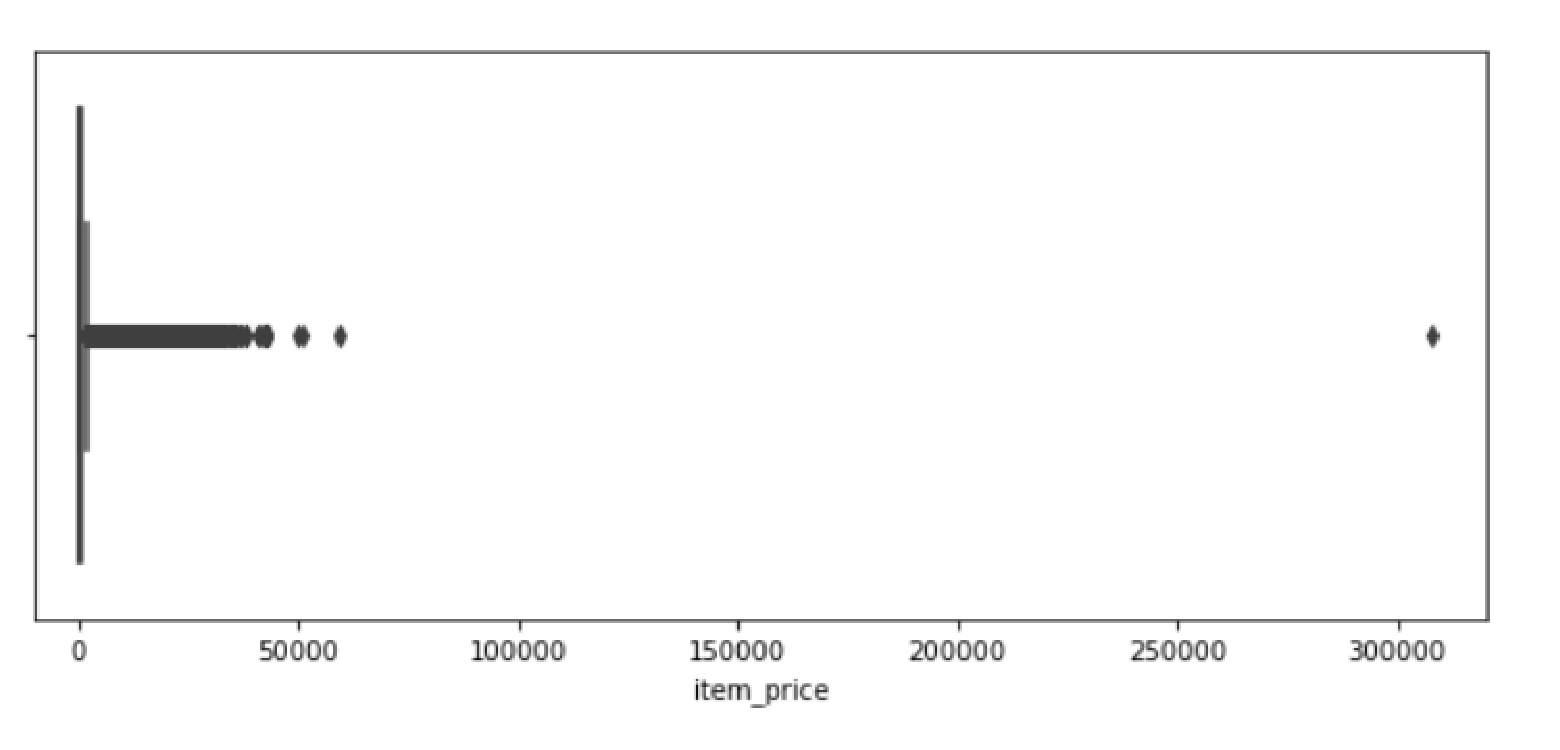
\includegraphics[scale=0.5]{picture/data_8.eps}
%DIFDELCMD <   \end{figure}
%DIFDELCMD < %%%
\DIFdelend \DIFaddbegin \twotonebox{\parbox{.1\textwidth}{result}}{\parbox{.76\textwidth}
  {
    \begin{figure}
      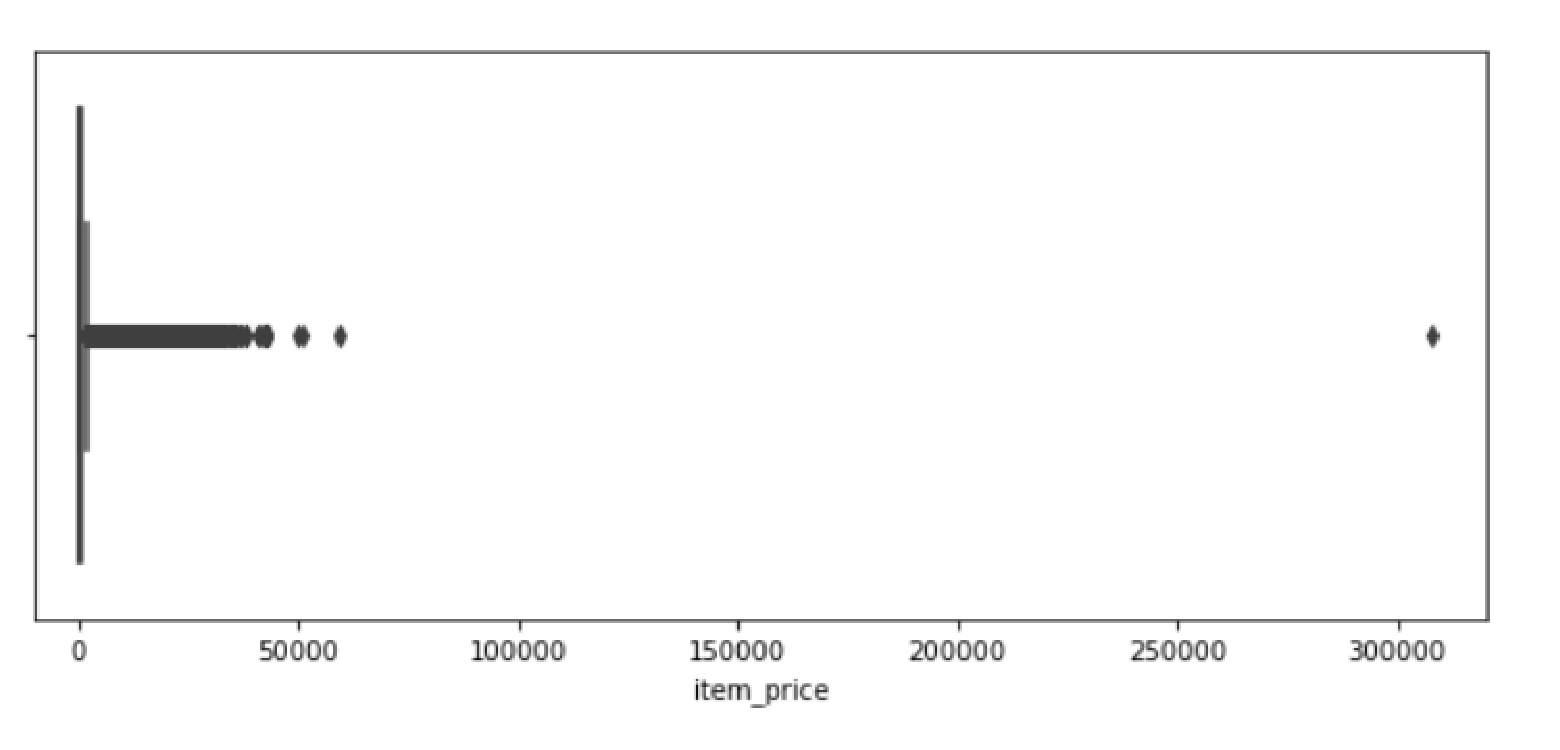
\includegraphics[scale=0.5]{picture/data_8.eps}
    \end{figure}
  }}
\DIFaddend \end{slide}
%%
%%==========================================================================================

%%==========================================================================================
%%
\DIFdelbegin %DIFDELCMD < \begin{slide}[toc=,bm=]{outdated items}
%DIFDELCMD <   %%%
\DIFdel{target:Analyze how many products have not been sold in the last six consecutive months. How many of these products appear in the test set.
  result:
  There are 12391 training sets, which have not been sold in the last six months.
  There are 164 test sets, which have not been sold in the last six months
}\DIFdelend \DIFaddbegin \begin{slide}[toc=,bm=]{outdated items and Negative}
  \twotonebox{\parbox{.1\textwidth}{target}}{\parbox{.76\textwidth}
  {
    Analyze how many products have not been sold in the last six consecutive months. How many of these products appear in the test set.
  }}

  \twotonebox{\parbox{.1\textwidth}{result}}{\parbox{.76\textwidth}
  {
    There are 12391 training sets, which have not been sold in the last six months.
    There are 164 test sets, which have not been sold in the last six months
  }}
  \bigskip

  \twotonebox{\parbox{.1\textwidth}{Negative}}{\parbox{.76\textwidth}
  {
    Change item whose commodity price is negative to median
  }}
\DIFaddend \end{slide}
%%
%DIF < %==
%DIF > %==========================================================================================

%%==========================================================================================
%%
\DIFdelbegin %DIFDELCMD < \begin{slide}[toc=,bm=]{Negative}
%DIFDELCMD <   %%%
\DIFdel{Change item whose commodity price is negative to median
  operation:
}\DIFdelend \DIFaddbegin \begin{slide}[toc=,bm=]{outdated items and Negative}  
  \twotonebox{\parbox{.1\textwidth}{Negative}}{\parbox{.76\textwidth}
  {
    Change item whose commodity price is negative to median
  }}
\DIFaddend \end{slide}
%%
%%==========================================================================================

\section{Data analysis}

%%==========================================================================================
%%
\begin{slide}[toc=,bm=]{Monthly sales of goods}
  \begin{figure}
    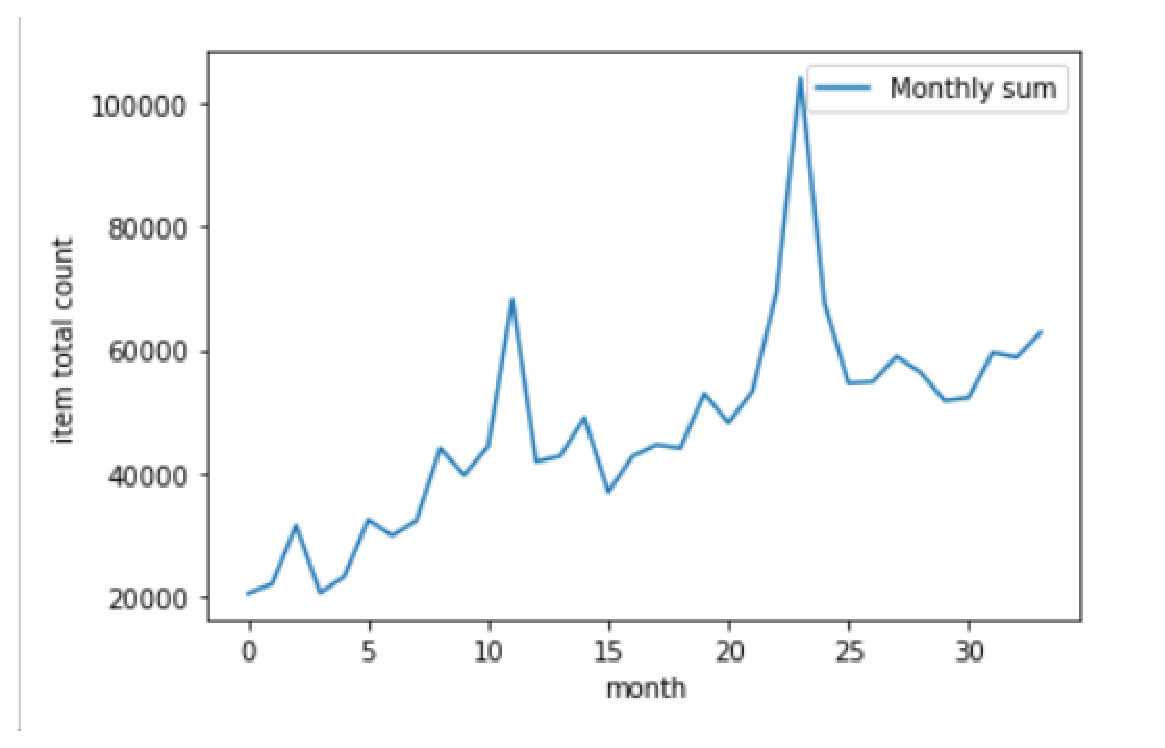
\includegraphics[scale=0.5]{picture/data_20.eps}
  \end{figure}
  \DIFaddbegin \begin{center}
    \textbf{\DIFadd{Figure 1}}\DIFadd{~~month_total_count.}\\
  \end{center}
    \DIFaddend Explain that the month is related to the sales volume of goods: the sales volume at the end of the year is increasing
\end{slide}
%%
%%==========================================================================================


%%==========================================================================================
%%
\begin{slide}[toc=,bm=]{Shop sales}
  \begin{figure}
    \DIFdelbeginFL %DIFDELCMD < 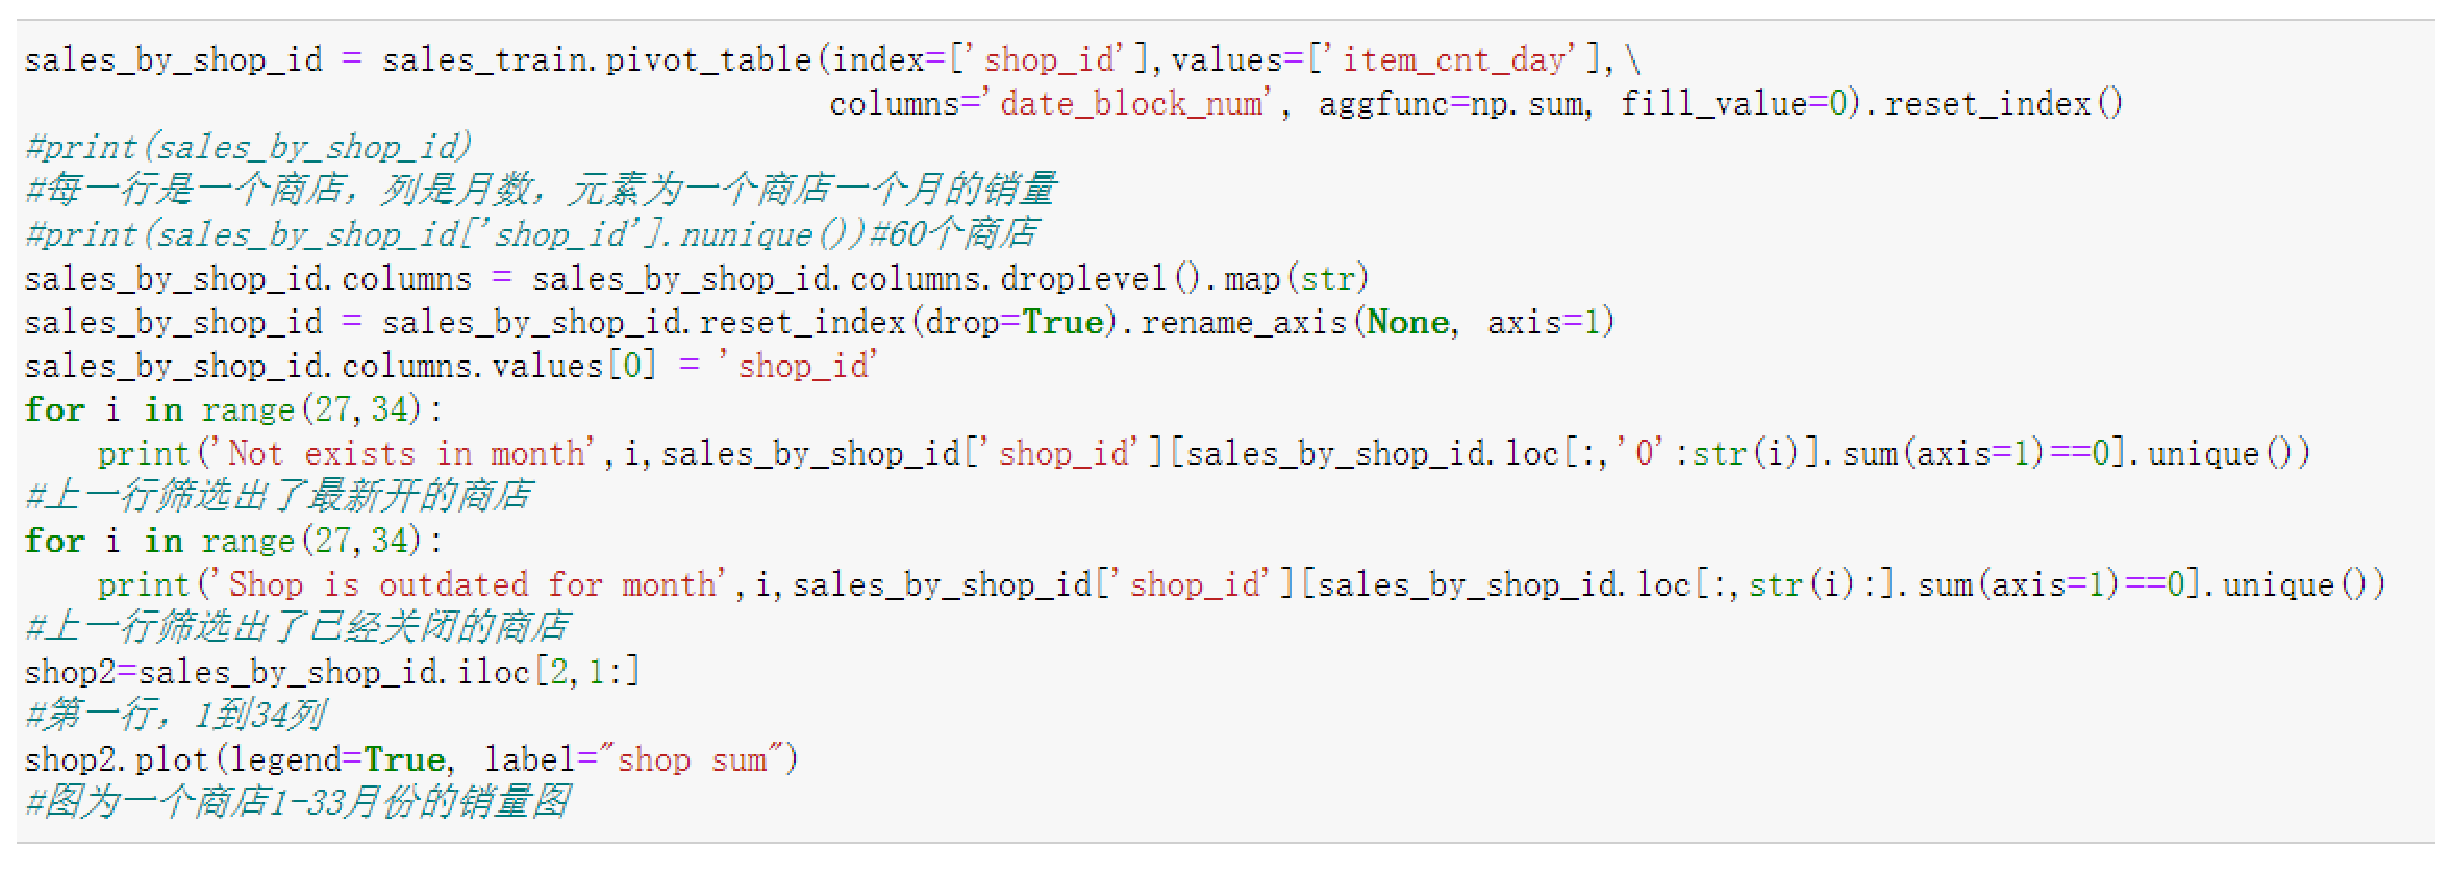
\includegraphics[scale=0.5]{picture/data_10.eps}
%DIFDELCMD <   %%%
\DIFdelendFL \DIFaddbeginFL 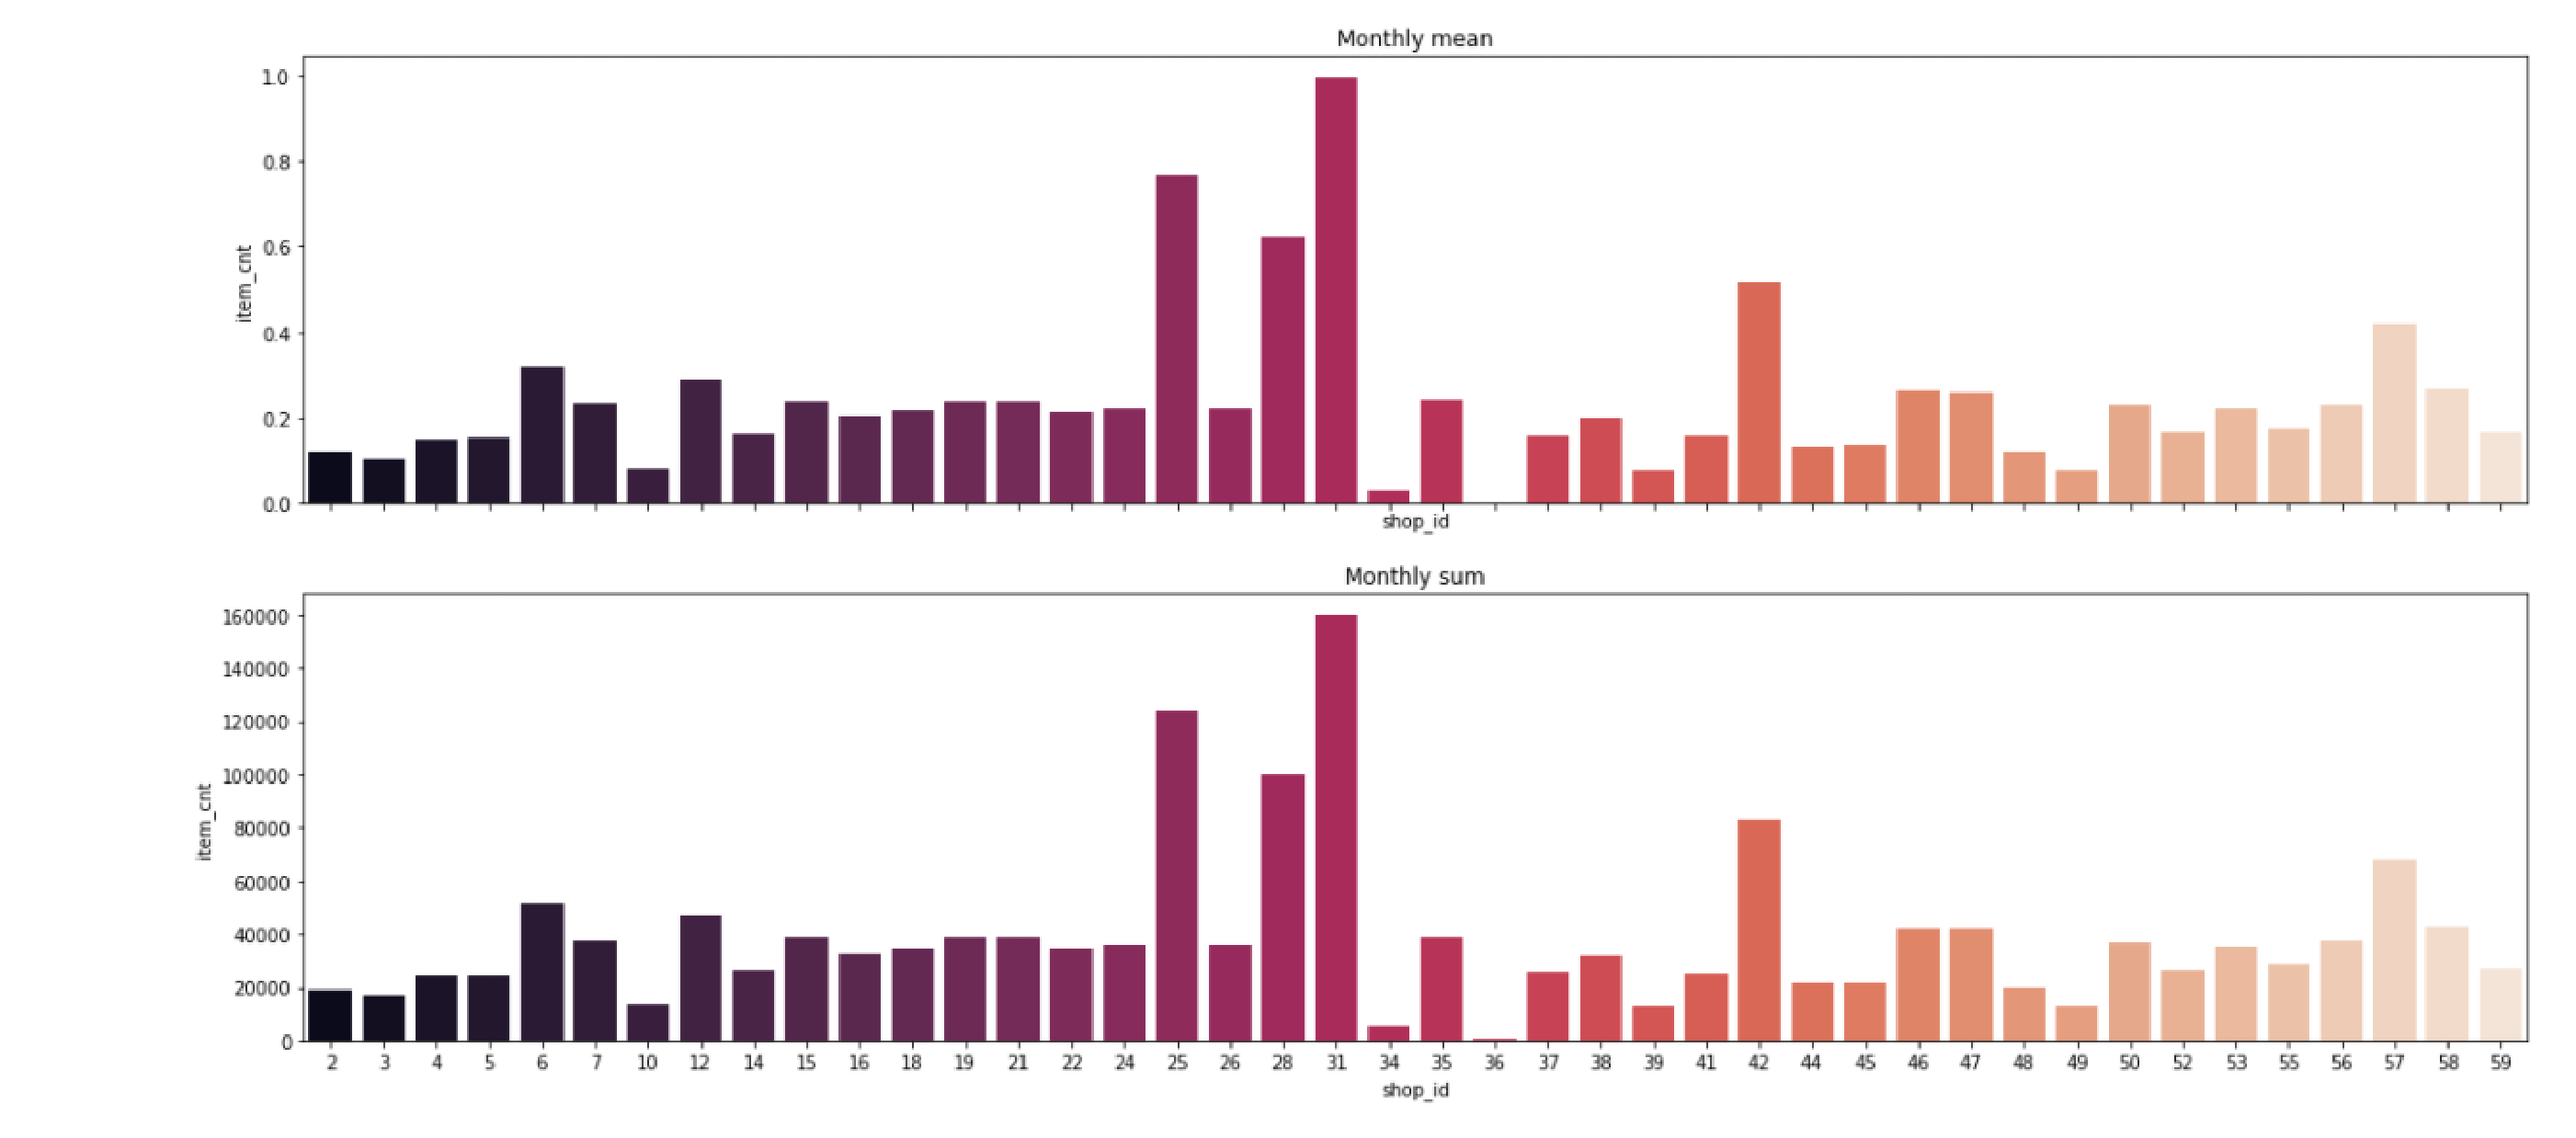
\includegraphics[scale=0.4]{picture/data_30.eps}
  \DIFaddendFL \end{figure}
  \begin{center}
    \DIFdelbegin \DIFdel{Objective: To prepare for feature extraction
  }\DIFdelend \DIFaddbegin \textbf{\DIFadd{Figure 2}}\DIFadd{~~shop_count.}\\
  \DIFaddend \end{center}
\end{slide}
%%
%%==========================================================================================

%%==========================================================================================
%%
\DIFdelbegin %DIFDELCMD < \begin{slide}[toc=,bm=]{Shop sales}
%DIFDELCMD <   %%%
\DIFdelend \DIFaddbegin \begin{slide}[toc=,bm=]{Sales of different category}
  \DIFaddend \begin{figure}
    \DIFdelbeginFL %DIFDELCMD < 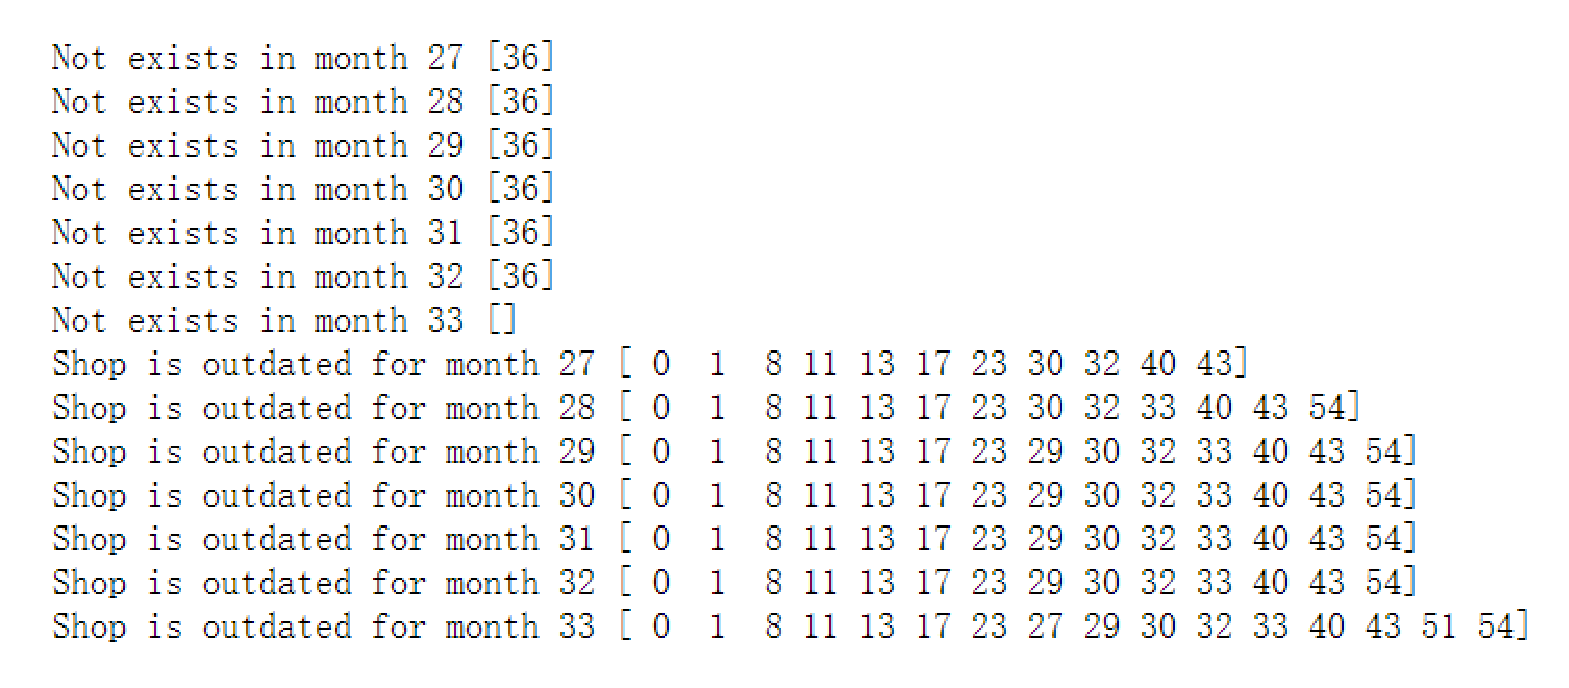
\includegraphics[scale=0.5]{picture/data_11.eps}
%DIFDELCMD <   %%%
\DIFdelendFL \DIFaddbeginFL 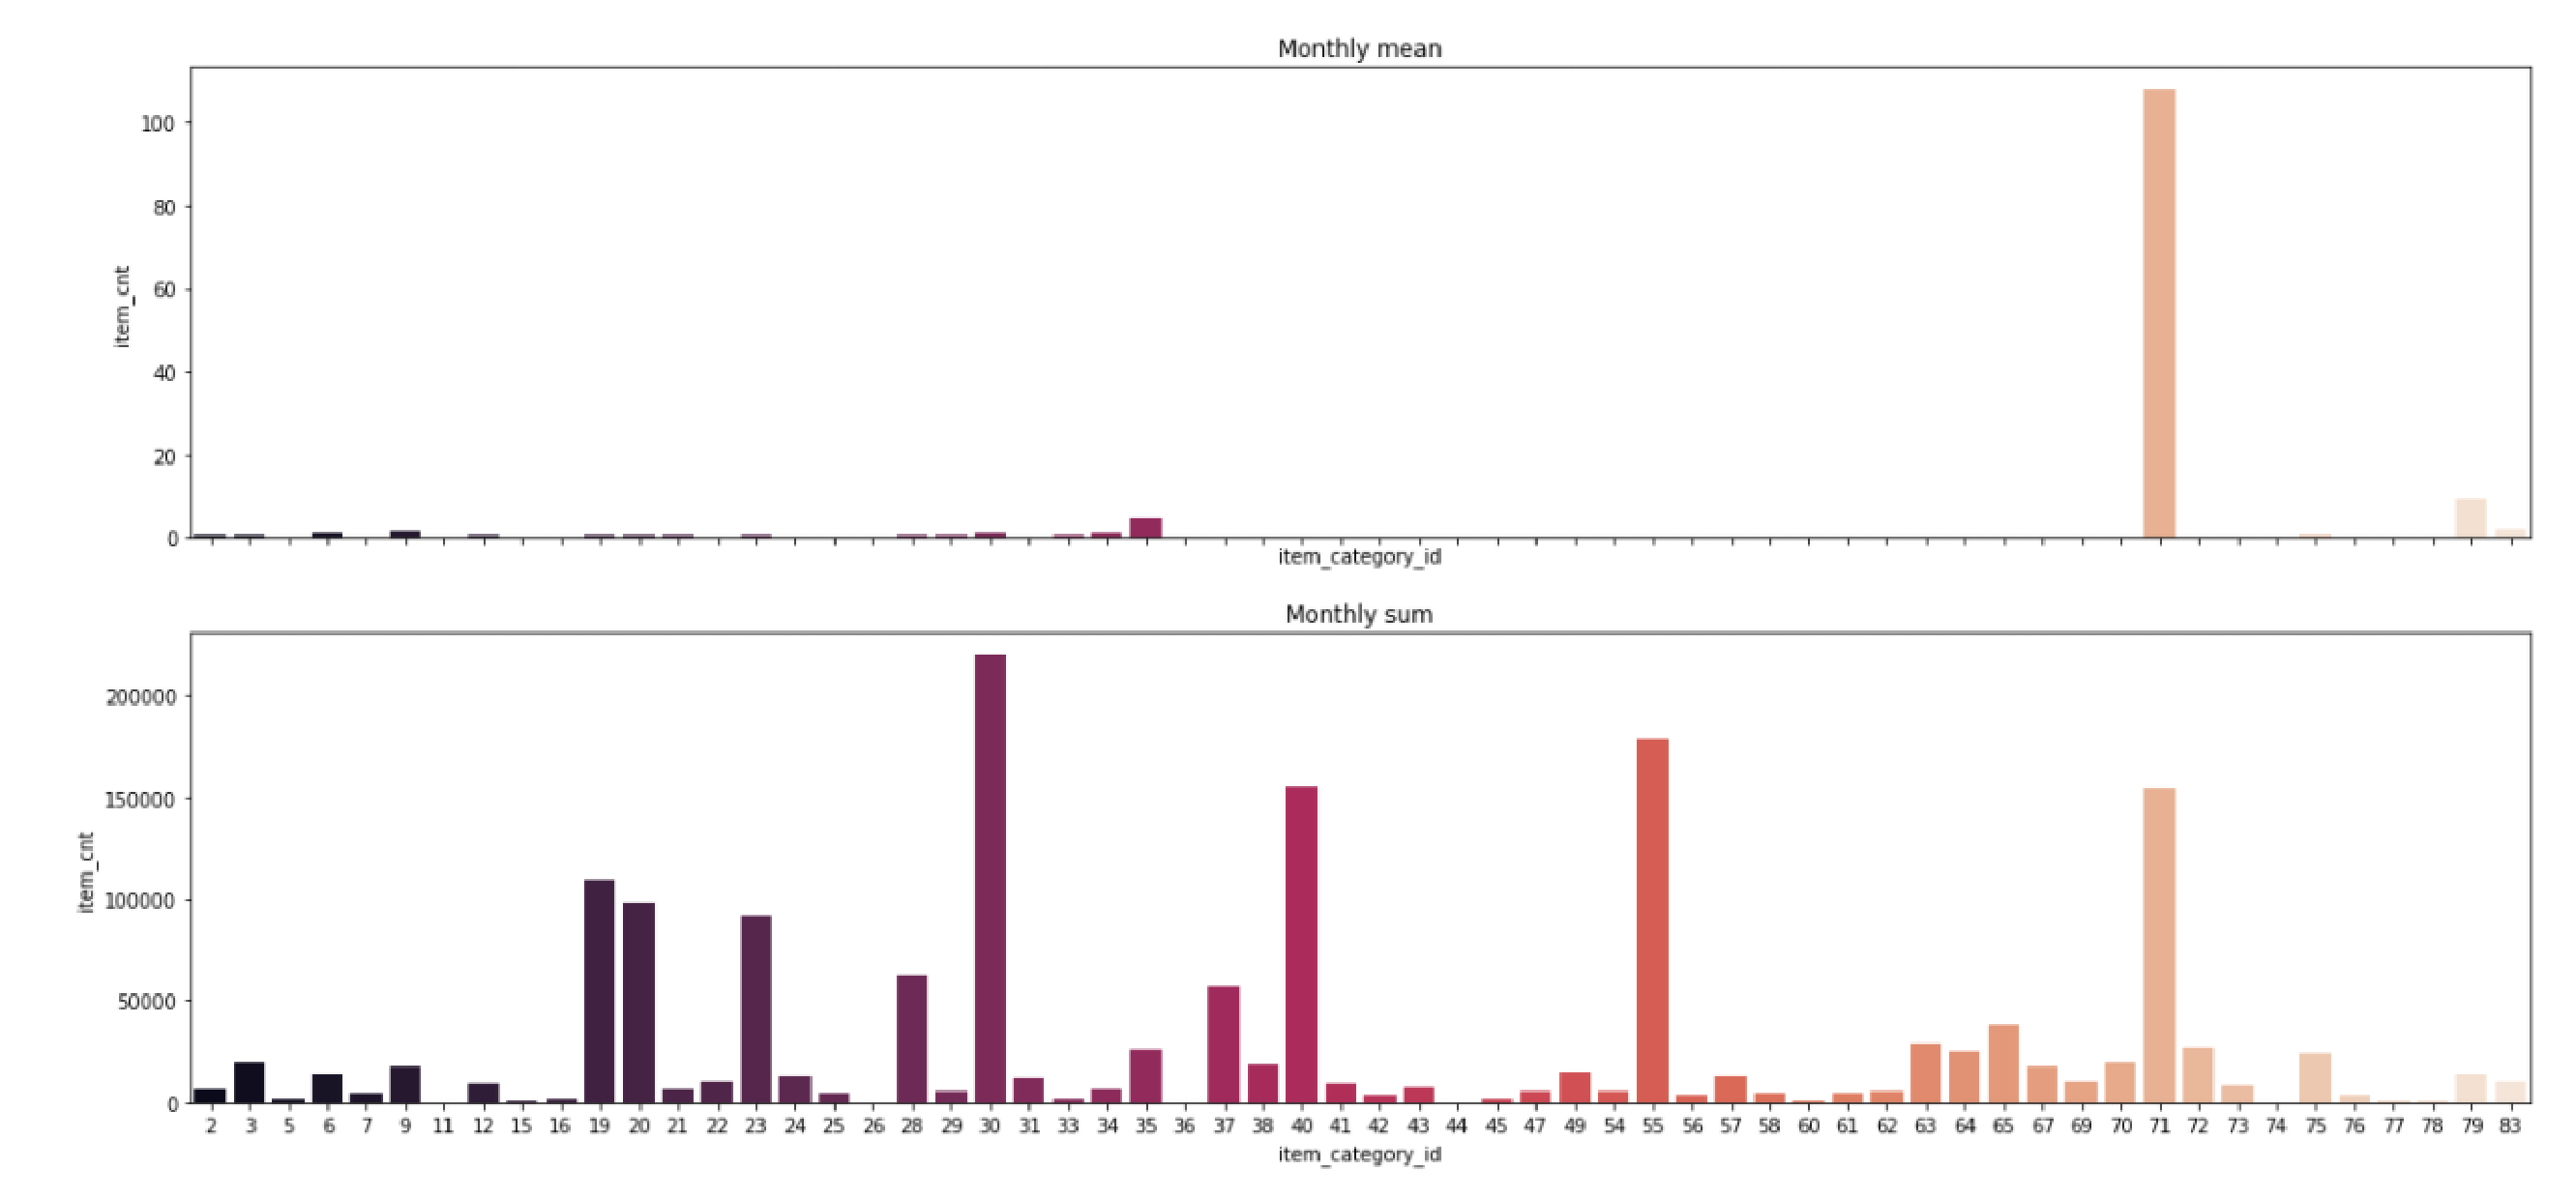
\includegraphics[scale=0.4]{picture/data_31.eps}
  \DIFaddendFL \end{figure}
  \DIFaddbegin \begin{center}
    \textbf{\DIFadd{Figure 3}}\DIFadd{~~item_category_count.}\\
  \end{center}
\DIFaddend \end{slide}
%%
%%==========================================================================================


%%==========================================================================================
%%
\DIFdelbegin %DIFDELCMD < \begin{slide}[toc=,bm=]{Item Information}
%DIFDELCMD <   %%%
\DIFdel{The categories of items are: large categories, small categories, we separate them, and code them separately to facilitate subsequent feature extraction
  }%DIFDELCMD < \begin{figure}
%DIFDELCMD <     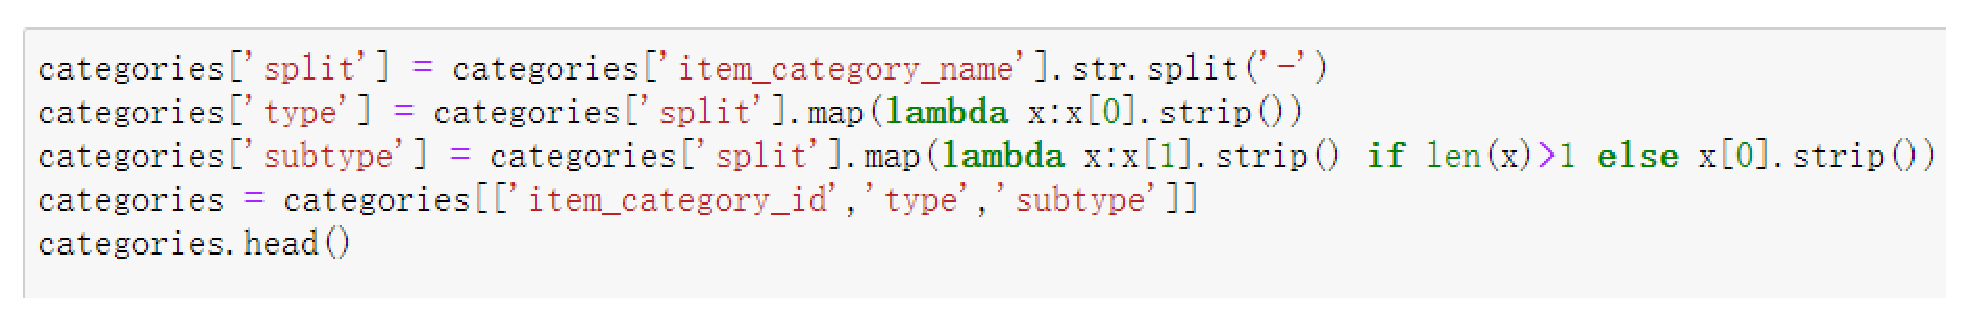
\includegraphics[scale=0.5]{picture/data_13.eps}
%DIFDELCMD <   \end{figure}
%DIFDELCMD < %%%
\DIFdelend \DIFaddbegin \begin{slide}[toc=,bm=]{Item and Shop Information}
  \twotonebox{\parbox{.1\textwidth}{categories of items}}{\parbox{.76\textwidth}
  {
    large categories, small categories, we separate them, and code them separately to facilitate subsequent feature extraction
  }}
  \twotonebox{\parbox{.1\textwidth}{Shop information}}{\parbox{.76\textwidth}
  {
    the city where the store is located, the type of store, which we separate and encode separately for subsequent feature extraction
  }}
\DIFaddend \end{slide}
%%
%%==========================================================================================

%DIF < %==========================================================================================
%DIF < %
\DIFdelbegin %DIFDELCMD < \begin{slide}[toc=,bm=]{Shop Information}
%DIFDELCMD <   %%%
\DIFdel{Shop information includes: the city where the store is located, the type of store, which we separate and encode separately for subsequent feature extraction
}%DIFDELCMD < \end{slide}
%DIFDELCMD < %%%
%DIF < %
%DIF < %==========================================================================================
\DIFdelend \DIFaddbegin \section{\DIFadd{Model}}
\DIFaddend 

%%==========================================================================================
%%
\DIFdelbegin %DIFDELCMD < \begin{slide}[toc=,bm=]{Shop Information}
%DIFDELCMD <   \begin{figure}
%DIFDELCMD <     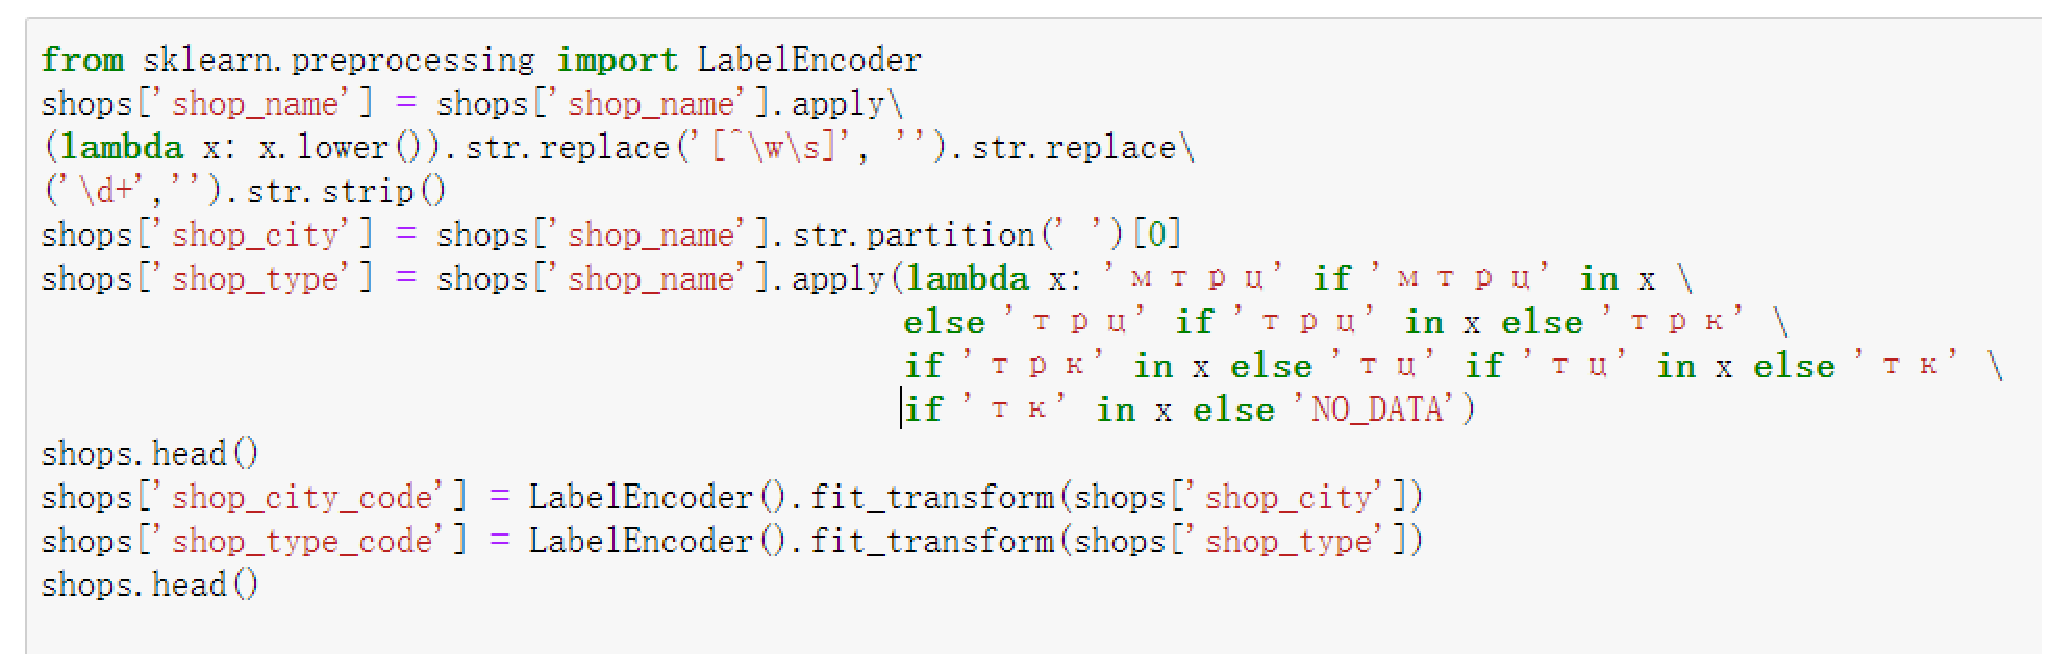
\includegraphics[scale=0.5]{picture/data_12.eps}
%DIFDELCMD <   \end{figure}
%DIFDELCMD < %%%
\DIFdelend \DIFaddbegin \begin{slide}[toc=,bm=]{decision tree}
  \twotonebox{\parbox{.1\textwidth}{Dicision tree}}{\parbox{.76\textwidth}
  {
    In machine learning, decision tree is a prediction model, which represents a mapping relationship between object attributes and object values. Each node in the tree represents an object, and each branch path represents a possible attribute value, while each leaf node corresponds to the value of the object represented by the path from the root node to the leaf node. The decision tree has only a single output, if you want to have complex output, you can establish an independent decision tree to deal with different outputs. Decision tree is a frequently used technology in data mining, which can be used to analyze data, and also can be used for prediction.
  }}
\DIFaddend \end{slide}
%%
%%==========================================================================================


%%==========================================================================================
%%
\DIFdelbegin %DIFDELCMD < \begin{slide}[toc=,bm=]{Items Information}
%DIFDELCMD <   %%%
\DIFdel{The training set contains only the items that the store actually sold that month,
  for items not sold during the month, you should add them and set them to 0
  }%DIFDELCMD < \begin{figure}
%DIFDELCMD <     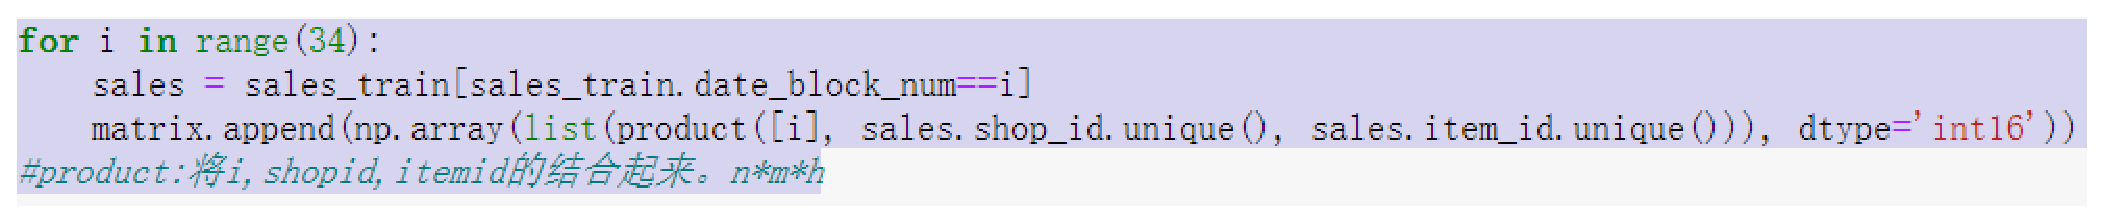
\includegraphics[scale=0.5]{picture/data_15.eps}
%DIFDELCMD <   \end{figure}
%DIFDELCMD <    %%%
\DIFdel{Cartesian product
}%DIFDELCMD < \end{slide}
%DIFDELCMD < %%%
%DIF < %
%DIF < %==========================================================================================
%DIFDELCMD < 

%DIFDELCMD < %%%
%DIF < %==========================================================================================
%DIF < %
%DIFDELCMD < \begin{slide}[toc=,bm=]{Monthly total sales}
%DIFDELCMD <  

%DIFDELCMD <   \begin{figure}
%DIFDELCMD <     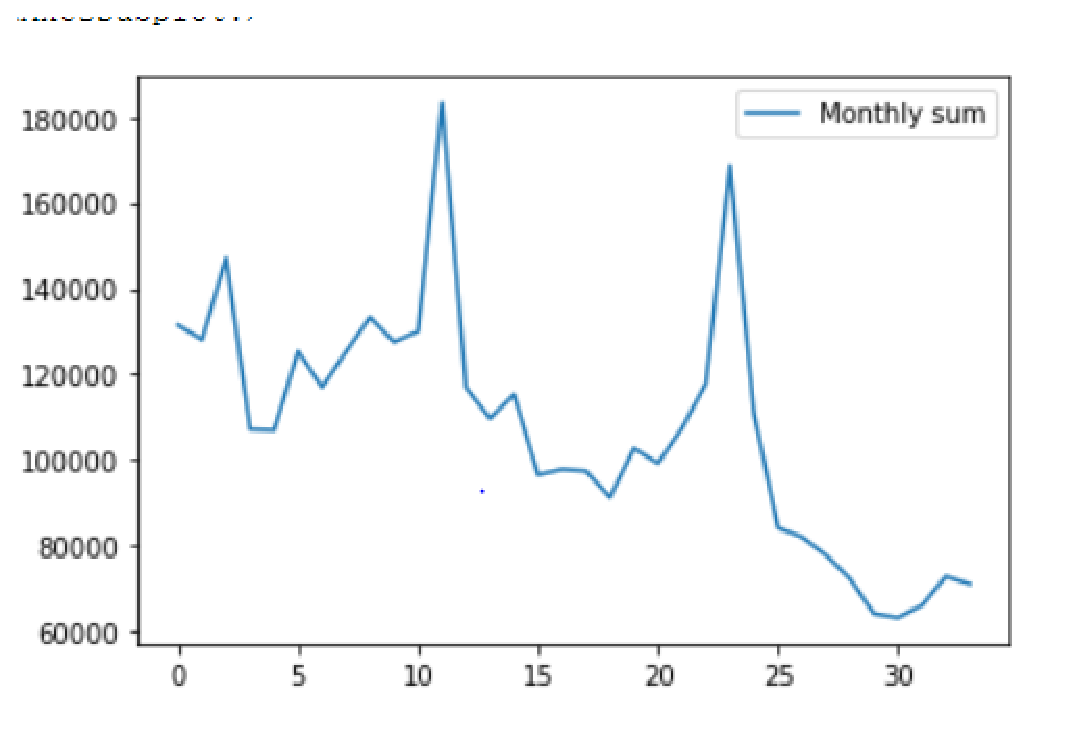
\includegraphics[scale=0.5]{picture/data_18.eps}
%DIFDELCMD <   \end{figure}
%DIFDELCMD < \end{slide}
%DIFDELCMD < %%%
%DIF < %
%DIF < %==========================================================================================
%DIFDELCMD < 

%DIFDELCMD < %%%
%DIF < %==========================================================================================
%DIF < %
%DIFDELCMD < \begin{slide}[toc=,bm=]{Sales per store}
%DIFDELCMD <   %%%
\DIFdel{It is known that the city to which the store belongs and the type of store affect sales
  }%DIFDELCMD < \begin{figure}
%DIFDELCMD <     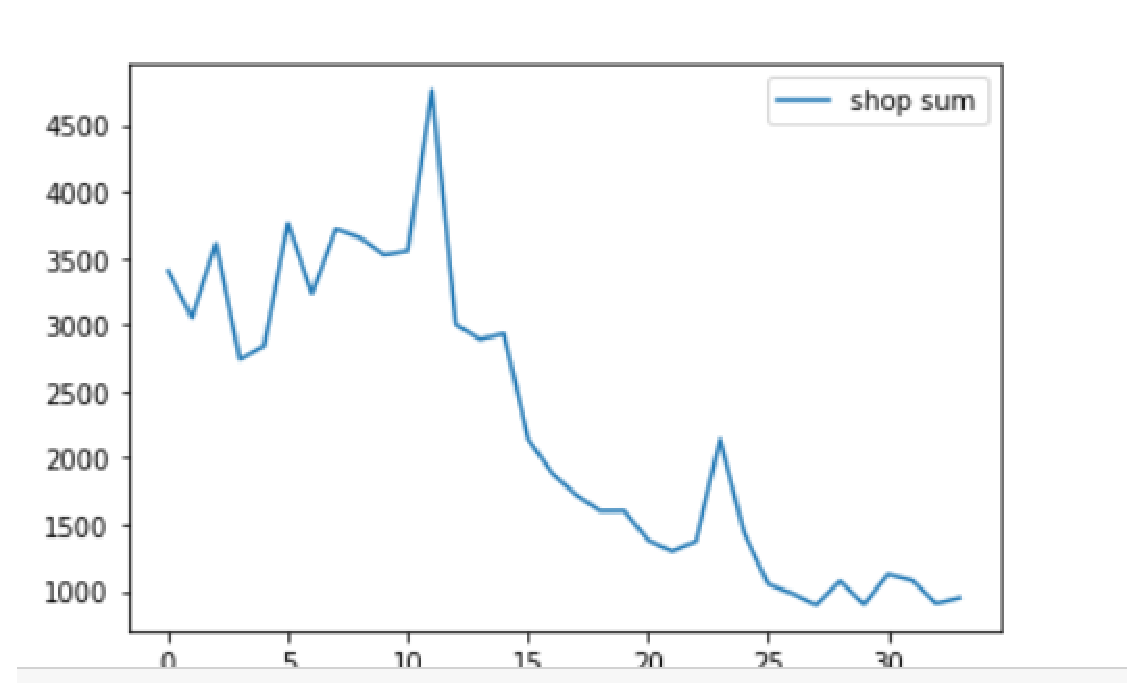
\includegraphics[scale=0.5]{picture/data_19.eps}
%DIFDELCMD <   \end{figure}
%DIFDELCMD < \end{slide}
%DIFDELCMD < %%%
%DIF < %
%DIF < %==========================================================================================
%DIFDELCMD < 

%DIFDELCMD < %%%
\section{\DIFdel{Model}}
%DIFAUXCMD
\addtocounter{section}{-1}%DIFAUXCMD
%DIFDELCMD < 

%DIFDELCMD < %%%
%DIF < %==========================================================================================
%DIF < %
\DIFdelend \begin{slide}[toc=,bm=]{Model selection}
  \begin{itemize}
    \item GBDT
    \item Xgboost
    \item lightgbm
    \item neural network
  \end{itemize}
\end{slide}
%%
%%==========================================================================================


%%==========================================================================================
%%
\begin{slide}[toc=,bm=]{Method One}
  \DIFdelbegin \DIFdel{Method:The sales of the 34th month are regarded as the sales of the 35th month}%DIFDELCMD < \par
%DIFDELCMD <   %%%
\DIFdel{operation:Count the sales volume of each item in each store in the 33rd month and merge it with test
  Result:RMSE=1.16777
}\DIFdelend \DIFaddbegin \twotonebox{\parbox{.1\textwidth}{Method}}{\parbox{.76\textwidth}
  {
    The sales of the 34th month are regarded as the sales of the 35th month
  }}
  \twotonebox{\parbox{.1\textwidth}{operation}}{\parbox{.76\textwidth}
  {
    Count the sales volume of each item in each store in the 33rd month and merge it with test
  }}
  \twotonebox{\parbox{.1\textwidth}{Result}}{\parbox{.76\textwidth}
  {
    RMSE=1.16777
  }}
\DIFaddend \end{slide}
%%
%%==========================================================================================


%%==========================================================================================
%%
\DIFdelbegin %DIFDELCMD < \begin{slide}[toc=,bm=]{Method One}
%DIFDELCMD <   %%%
\DIFdel{features:shop_id,item_id,item_cnt_month}%DIFDELCMD < \par
%DIFDELCMD <   %%%
\DIFdel{Method:lightgbm
  }%DIFDELCMD < \begin{figure}
%DIFDELCMD <     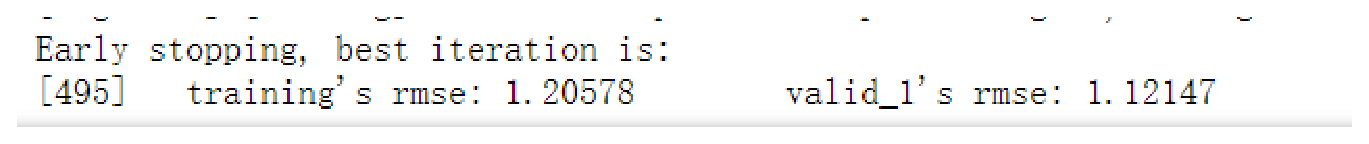
\includegraphics[scale=0.5]{picture/data_14.eps}
%DIFDELCMD <   \end{figure}
%DIFDELCMD <   %%%
\DIFdel{attention:After some data preprocessing
}%DIFDELCMD < \end{slide}
%DIFDELCMD < %%%
%DIF < %
%DIF < %==========================================================================================
%DIFDELCMD < 

%DIFDELCMD < %%%
%DIF < %==========================================================================================
%DIF < %
\DIFdelend \begin{slide}[toc=,bm=]{Method Two}
  \DIFdelbegin \DIFdel{Some historical information needs to be generated by delayed operations. For example, you can use the 0-33 month sales as a historical feature of the 1-34 month (one month delay).
}\DIFdelend \DIFaddbegin \twotonebox{\parbox{.1\textwidth}{Features}}{\parbox{.76\textwidth}
  {
    \begin{itemize}
      \item shop_id
      \item item_id
      \item item_cnt_month
    \end{itemize}
  }}
  \twotonebox{\parbox{.1\textwidth}{Method}}{\parbox{.76\textwidth}
  {
    lightgbm
  }}
  \twotonebox{\parbox{.1\textwidth}{Result}}{\parbox{.76\textwidth}
  {
    RMSE=
  }}
\DIFaddend \end{slide}
%%
%%==========================================================================================

%%==========================================================================================
%%
\DIFdelbegin %DIFDELCMD < \begin{slide}[toc=,bm=]{Method Two}
%DIFDELCMD <   \begin{itemize}

%DIFDELCMD < \end{itemize}
%DIFDELCMD < %%%
\DIFdelend \DIFaddbegin \begin{slide}[toc=,bm=]{Method Three}
  \twotonebox{\parbox{.1\textwidth}{Data feature}}{\parbox{.76\textwidth}
  {
    'date_block_num', 'shop_id', 'item_id', 'item_category_id', 'cat_type_code', 'cat_subtype_code', 'shop_city_code', 'shop_type_code'
  }}
  \twotonebox{\parbox{.1\textwidth}{Monthly sales feature}}{\parbox{.76\textwidth}
  {
    \begin{itemize}
      \item item_cnt_month
      \item date_avg_item_cnt
      \item date_item_avg_item_cnt
      \item date_shop_avg_item_cnt
      \item date_cat_avg_item_cnt
      \item date_cat_shop_avg_item_cnt
      \item date_type_avg_item_cnt
      \item date_item_type_avg_item_cnt
      \item date_city_avg_item_cnt
   \end{itemize}
  }}
  \twotonebox{\parbox{.1\textwidth}{Historical feature}}{\parbox{.76\textwidth}
  {
    delay:1,2,3,6,12
  }}
\DIFaddend \end{slide}
%%
%%==========================================================================================

%%==========================================================================================
%%
\DIFdelbegin %DIFDELCMD < \begin{slide}[toc=,bm=]{Method Two}
%DIFDELCMD <   %%%
\DIFdelend \DIFaddbegin \begin{slide}[toc=,bm=]{Method Three}
  \DIFaddend \begin{figure}
    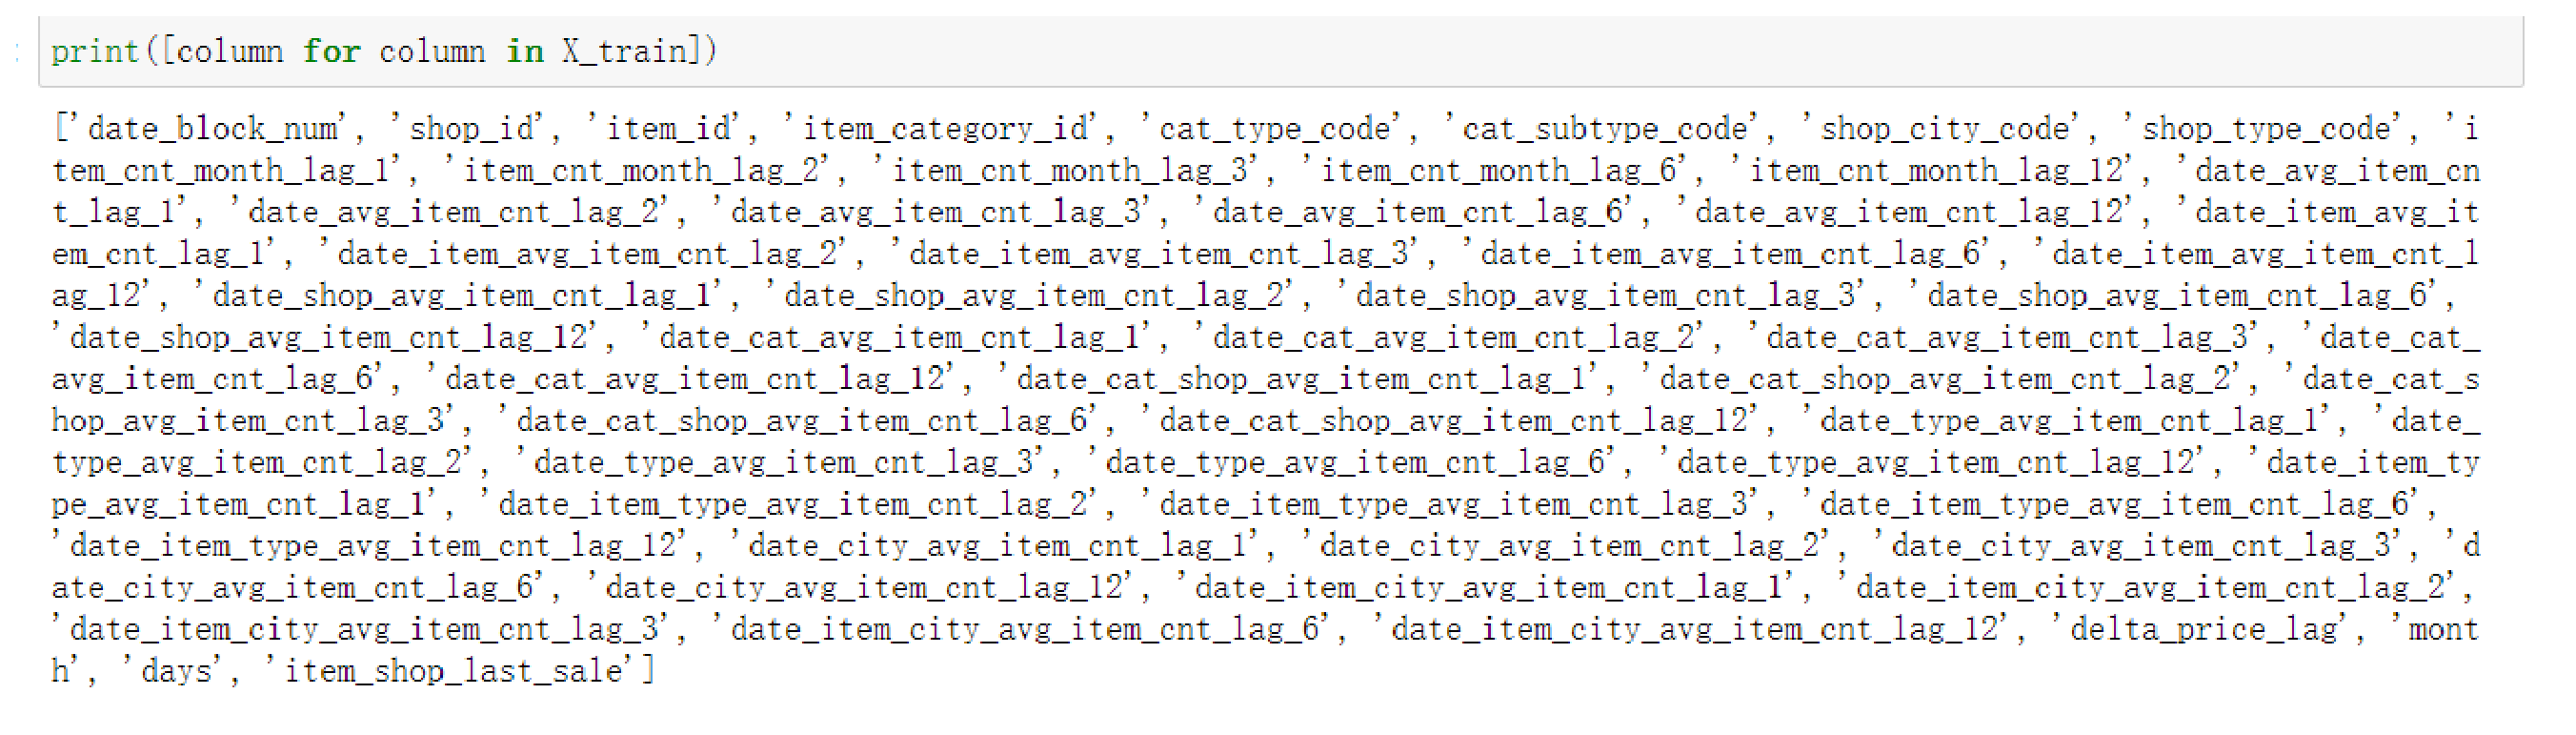
\includegraphics[scale=0.5]{picture/data_16.eps}
  \end{figure}
\end{slide}
%%
%%==========================================================================================

%%==========================================================================================
%%
\DIFdelbegin %DIFDELCMD < \begin{slide}[toc=,bm=]{Method Two}
%DIFDELCMD <   \begin{figure}
%DIFDELCMD <     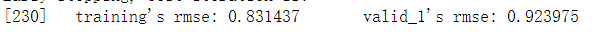
\includegraphics[scale=0.5]{picture/data_17.eps}
%DIFDELCMD <   \end{figure}
%DIFDELCMD < %%%
\DIFdelend \DIFaddbegin \begin{slide}[toc=,bm=]{Method Three}
  \twotonebox{\parbox{.1\textwidth}{Result}}{\parbox{.76\textwidth}
  {\begin{itemize}
    \item training's rmse: 0.664209
    \item valid_1's rmse: 0.880256
  \end{itemize}
  }}
\DIFaddend \end{slide}
%%
%%==========================================================================================

\section{Lightgbm}

\end{document}
